\documentclass[a4paper,10pt,titlepage]{article}
% Språk och encodings
\usepackage[swedish,english]{babel}
\usepackage[T1]{fontenc}
\usepackage[utf8]{inputenc}
\usepackage[fixlanguage]{babelbib}
% Images and floats
\usepackage{graphicx}
\usepackage{wrapfig}
\usepackage{float}
% Clear type + Sans-serif font
\usepackage{lmodern}
\renewcommand{\familydefault}{\sfdefault}
% Avancerade tabeller
\usepackage{tabularx}
\usepackage{multirow}
\usepackage{booktabs}
% Matte
\usepackage{amsmath, amsthm, amssymb}
% Algoritmer
\usepackage[ruled,vlined]{algorithm2e}
% Källkod
\usepackage{listings}
\lstset{
	showspaces = false,
	showstringspaces = false,
}
% Inkludera pdf-sidor
\usepackage{pdfpages}
% Länkar
\usepackage{color}
\definecolor{dark-blue}{rgb}{0, 0, 0.6}
\usepackage{hyperref}
\hypersetup{
  colorlinks=true,
  linkcolor=dark-blue,
  urlcolor=dark-blue
}
% Vettiga paragrafer
\setlength{\parindent}{0pt}
\setlength{\parskip}{2ex}

% Kommando för kommandorader
\newcommand{\cmdline}[1]{\mbox{\textbf{\texttt{> #1}}}}

% Kommandon för testfall
\usepackage{testcases}

% Sidhuvud/sidfot
\usepackage{fancyhdr}
\setlength{\headheight}{15pt}
\pagestyle{fancyplain}
\lfoot{Carl-Oscar Erneholm \\ 880422-0872 \\ coer@kth.se}
\rfoot{Martin Nycander \\ 881028-0076 \\ mnyc@kth.se}
\cfoot{Sida \thepage}

% Språk
\selectbiblanguage{swedish}
\selectlanguage{swedish}

% Titel
\title{Laborationsrapport 3 \\ Minneshantering v. 3.21}
\author{Carl-Oscar Erneholm \and Martin Nycander}
\date{\today}

\begin{document}

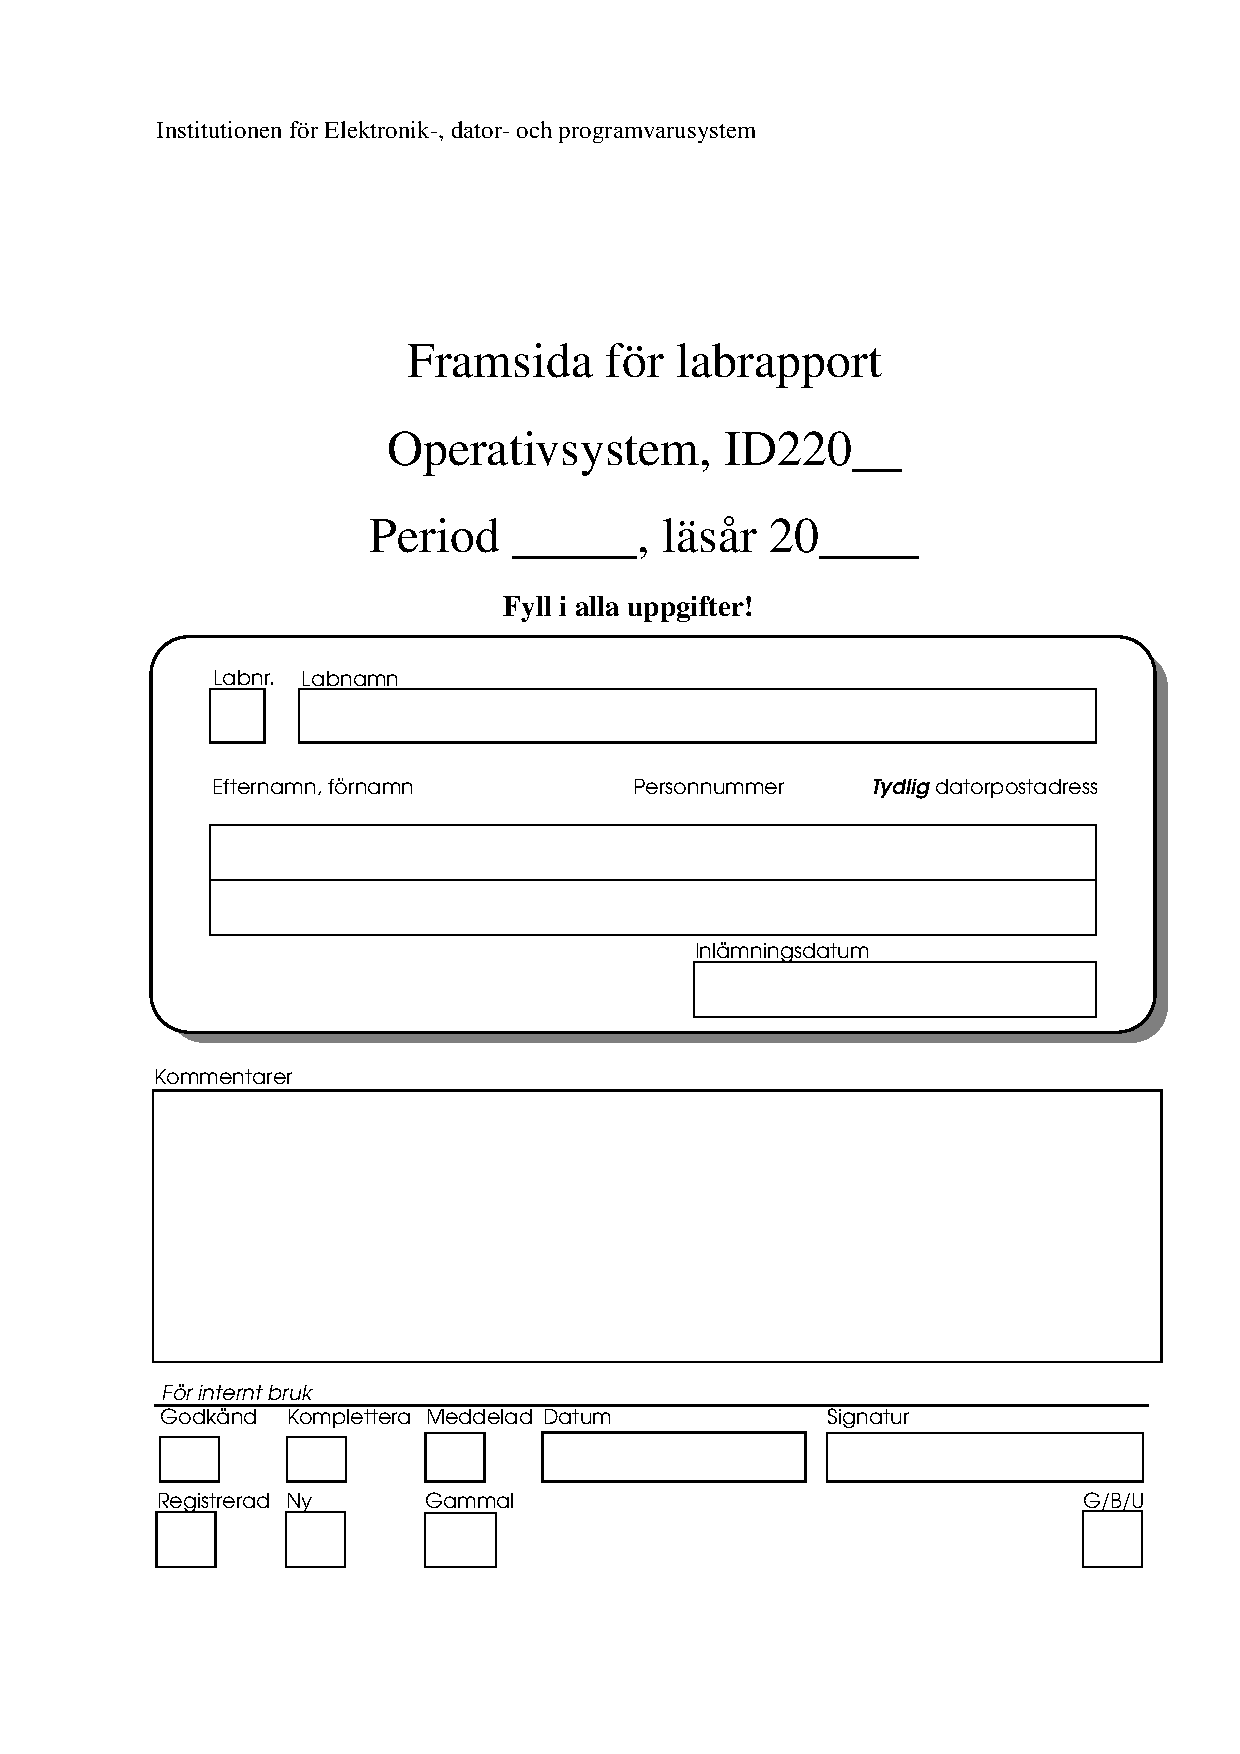
\includepdf[pages=-]{framsida.pdf}

\maketitle

\tableofcontents
\thispagestyle{empty}
\newpage
\setcounter{page}{1}
\section{Problembeskrivning}

De olika minnesallokeringsmetoderna som ska implementeras är:

\begin{description}
	\item[First-fit] Första bästa tillräckligt stora blocket används.
	\item[Best-fit] Det minsta lediga blocket med tillräckligt många bytes allokeras.
	\item[Worst-fit] Det största lediga blocket används och fragmenteras.
	\item[Quick-fit] Som Best-fit, men istället för att alla block kontrolleras så har man ett antal listor med minne av olika storlek.
\end{description}

Dessa ska implementeras i enlighet med hjälp av ett antal givna acceptanstest.

Vidare ska även samtliga algoritmers prestanda utvärderas utförligt i några väl valda aspekter.

\subsection{Förberedelsefråga}

\begin{enumerate}
\item[1.] \textbf{\footnotesize Hur mycket minne slösas bort i medel och i värsta fallet i de block som allokeras via malloc() ur ``Quick fit'' listorna?}

Quick fit listorna tar emot block av jämna två potenser av ett
förutbestämt värde. Det betyder att den tillåtna blockstorleken i
varje lista dubblas för varje lista ända tills den sista listan. I
det värsta fallet får ett block precis inte plats i ett en lista utan är en
enhet för stor, vilket betyder att den måste placeras i listan för dubbelt så
stora block.

\begin{equation*}
\begin{array}{c}
n+1 > n\\
2n - (n+1)\\
n-1\\
\frac{n-1}{2n} \approx \frac{1}{2}\\
\end{array}
\end{equation*}

Där $n$ är storleken på blocket där minnet inte fick plats.
Eftersom minnet vi ville allokera bara är något större än det block den inte
fick plats i är den mycket nära hälften så stor nästa lista med dubbelt så många
block. Alltså spiller vi i värsta fall nästan $50\%$ av allt vi allokerar.

Medelvärdet av minnes spillet när man använder Quick Fit ökar när block
storleken ökar (man har fler listor som tillåter större block). Den största
andelen spill kommer att komma ifrån de större block listorna, eftersom dem har
mer minne att spilla. Medelvärdet kommer alltså att domineras av de större
blockstorlekarna. De större blockstorlekarna kommer dessutom att ha ett mycket
snarlikt medelvärde, alltså kan vi approximera hela medelvärdet till medelvärdet
hos listan med störst block. Medelvärdet av minnesspillet i den sista listan är:

\begin{equation*}
\sum^n_{i=1}\frac{i}{n} = \frac{n + 1}{2}
\end{equation*}
\begin{equation*}
\frac{\frac{n + 1}{2}}{n} = \frac{n+1}{2n} = \frac{1}{2} + \frac{1}{2n}
\end{equation*}

Där $n$ är storleken på det blocken i den sista listan. Det slutgiltiga uttrycket
för andelen minnesspill $\frac{1}{2} + \frac{1}{2n}$ består av två
termer: $\frac{1}{2}$ som är värsta fallet ($50\%$) och $\frac{1}{2n}$, när $n$
ökar kommer den andra termen minska i värde och uttrycket kommer närma sig värstafallet. 
Medelfallet kommer i praktiken tyvärr att ligga ganska nära värstafallet $50\%$ spill.

\end{enumerate}

\newpage
\section{Programbeskrivning}

Programstrukturen var given i uppgiftsbeskrivningen, vi kompletterade den en del med hjälp av man-sidorna för malloc/free/realloc.
De ändringar vi gjorde var att i \texttt{malloc.c} ha en preprocessorvillkorssats som inkluderade de olika algoritmerna beroende på vad \texttt{STRATEGY} var satt till. Baskoden togs direkt från boken ``The C Programming Language'' precis som det tipsades om i boken, den koden ligger till grund för den större delen av våra implementationer.

Vi hade problem med hur sorteringen skulle gå till i best/worst fit. Frågan var om man skulle försöka hålla listan sorterad in-place eller sortera om den varje gång. Men efter mycket om och men kom vi fram till att det var ingen stor förlust att sortera om listan efter varje operation från början.

Implementeringen var sedan ganska rakt på. Gick något fel fick man använda sig av `gdb' för att stega sig igenom programmet och inspektera variabler. I slutet kontrollerades beteendet med hjälp av testfallen.

\newpage
\section{Prestandautvärdering}

% TODO: Använd testcases för att standardisera hur prestandamätningen görs

Vi har valt att utföra två huvudtester; ett som mäter tidsprestanda och ett som mäter andelen overhead.

\subsection{Tid}

Vi mäter tiden det tar att köra ett antal varierande \texttt{malloc} resp. \texttt{free} med hjälp av unix-kommandot \texttt{`time'}.


\subsubsection{Testkod}

Koden som kördes vid tillfällena visas här:

\scriptsize{\lstinputlisting[language=C]{../program/performance/time.c}}
\normalsize

\subsubsection{Resultat}

Nedan finnes resultat av tidskörningarna.
\begin{figure}[H]
	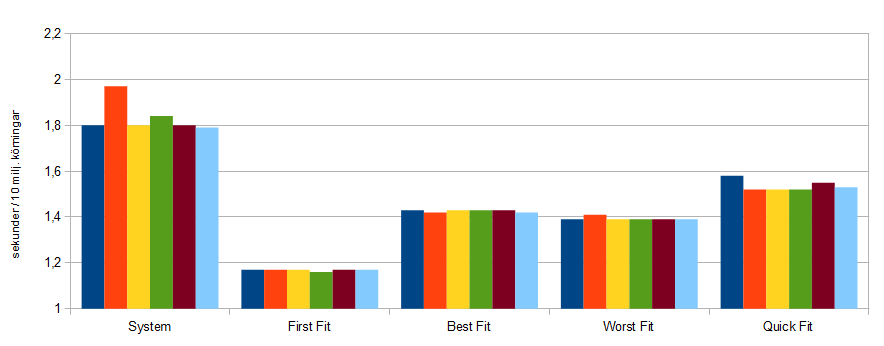
\includegraphics[width=\textwidth]{time.png}
	\caption{Resultat från 5 körningar av de olika algoritmerna.}
\end{figure}
\begin{tabular}{| l | c | c | c | c | c | c | c |}
		\hline
		 & Körn. 1	& Körn. 2	& Körn. 3	& Körn. 4	& Körn. 5	& Körn. 6	& Std. avvikelse. \\
		\hline
		System		& 1,8 s			& 1,97 s	& 1,8 s		& 1,84 s	& 1,8 s		& 1,79 s	& 0,07 s \\
		First Fit	& 1,17 s		& 1,17 s	& 1,17 s	& 1,16 s	& 1,17 s	& 1,17 s	& 0,00 s \\
		Best Fit	& 1,43 s		& 1,42 s	& 1,43 s	& 1,43 s	& 1,43 s	& 1,42 s	& 0,01 s \\
		Worst Fit	& 1,39 s		& 1,41 s	& 1,39 s	& 1,39 s	& 1,39 s	& 1,39 s	& 0,01 s \\
		Quick Fit	& 1,58 s		& 1,52 s	& 1,52 s	& 1,52 s	& 1,55 s	& 1,53 s	& 0,02 s \\
		\hline
\end{tabular}

Vi kan utläsa att den enklaste algoritmen, `First Fit` är den snabbaste. Best och Worst fit har mer logik och kräver därför mer tid på sig. Långsammast, vilket är lite motsägelsefullt var `Quick Fit`. Detta beror på att våran Quick fit implementation aldrig förallokerar några block, utan bara allokerar så mycket som behövs. Just denna testkod är lite orättvis eftersom bara tre block allokeras åt gången, quick-fit listornas fördelar utnyttjas aldrig med så få block.


Sammanfattningsvis kan man se att vi ligger under systemets egna tidsåtgång, vilket betyder att vi egentligen inte har några prestandaproblem i just det här fallet.

\subsection{Overhead}

Vi använder tre olika storlekar för mätdata en liten (64 bytes), en stor (10 sidor) och en slumpmässig (0 till 2 sidor). Dessa har allokerats 1000 gånger. Den faktiska åtgången har mäts m.h.a \texttt{sbrk(0)} och den optimala åtgången har även summerats. Dessa har dividerats för att få en faktor på hur stor del av datan som är overhead.

\subsubsection{Testkod}

\scriptsize{\lstinputlisting[language=C]{../program/performance/memory.c}}
\normalsize

\subsubsection{Resultat}

\begin{figure}[H]
	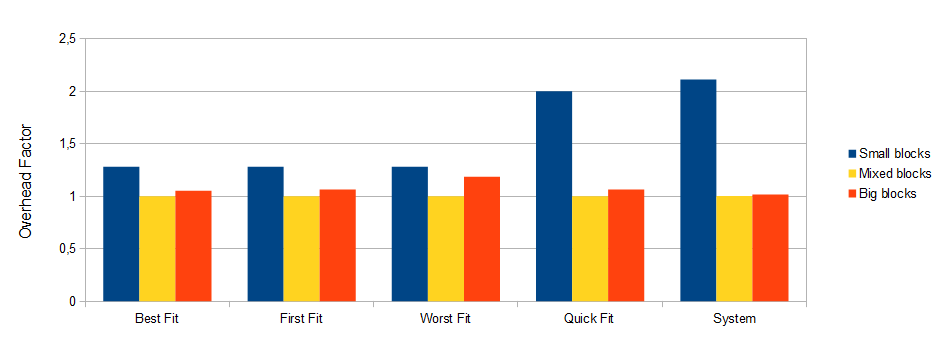
\includegraphics[width=\textwidth]{overhead.png}
\end{figure}

\begin{center}

	\begin{tabular}{ | >{\bfseries}l | c | c | c | r |}
		\hline
					& Small blocks	& Big blocks	& Mixed blocks	& Avg \\
		\hline
		Best Fit	& 1,28	& 1,0004	& 1,051		& 1,110 \\
		First Fit	& 1,28	& 1,0004	& 1,0631	& 1,114 \\
		Worst Fit	& 1,28	& 1,0004	& 1,1854	& 1,155 \\
		Quick Fit	& 2		& 1,0004	& 1,0631	& 1,355 \\
		System		& 2,112	& 1,0006	& 1,0169	& 1,377 \\
		\hline
	\end{tabular}
\end{center}

Som väntat kan vi se att Quick Fit är slösaktig med minnet. Systemets egna malloc hamnar i dåligt läge på grund av den dåliga presteringen för små block. Vidare kan vi konstantera att för stora block är overhead-datan obetydlig, som sig bör.

Vi kan även se att för stora block så är quick fit ekvivalent med first fit, precis som den ska eftersom alla block hamnar i den sista listan.



\newpage
\section{Labbutvärdering}

Labben hade en klart annorlunda struktur är de tidigare labbarna. Nedan följer lite reflektioner kring laborationen:

\begin{itemize}
	\item Att leverera färdiga tester istället för en kravspec är en klar förbättring och gör utvecklingen mycket enklare.
	\item Labben tvingade oss att använda och förstå debuggaren `gdb' för att hitta fel. En övning om enbart gdb hade nog varit grymt, ty den är inte särskilt intuitiv att använda.
	\item Att ha 4 skilda algoritmer gjorde det lätt att arbeta parallellt.
\end{itemize}

Estimerat nedlagd tid: $1 \text{ arbetsvecka} \cdot 2 \text{ personer}$. \\
Svårighetsgrad: $4/5$.

\end{document}
